\documentclass[fleqn, a4paper, 12pt, oneside]{amsart}
\usepackage{exsheets}
\usepackage{amsmath, amssymb, amsthm} %standard AMS packages
\usepackage{marginnote} %marginnotes
\usepackage{gensymb} %miscellaneous symbols
\usepackage{commath} %differential symbols
\usepackage{xcolor} %colours
\usepackage{cancel} %cancelling terms
\usepackage{siunitx} %formatting units
\usepackage{tikz, pgfplots} %diagrams
\usetikzlibrary{calc, hobby, patterns, intersections}
\usepackage{graphicx} %inserting graphics
\usepackage{hyperref} %hyperlinks
\usepackage{datetime} %date and time
\usepackage{ulem} %underline for \emph{}
\usepackage{xfrac} %inline fractions
\usepackage{enumerate} %numbered lists
\usepackage{float} %inserting floats
\usepackage{circuitikz} %circuit diagrams

\newcommand\numberthis{\addtocounter{equation}{1}\tag{\theequation}} %adds numbers to specific equations in non-numbered list of equations

\newcommand{\AxisRotator}[1][rotate=0]{
	\tikz [x=0.25cm,y=0.60cm,line width=.2ex,-stealth,#1] \draw (0,0) arc (-150:150:1 and 1);%
} %rotation symbols on axes

\theoremstyle{definition}
\newtheorem{example}{Example}
\newtheorem{definition}{Definition}

\theoremstyle{theorem}
\newtheorem{theorem}{Theorem}

\newcommand{\curl}{\mathrm{curl\,}}

\makeatletter
\@addtoreset{section}{part} %resets section numbers in new part
\makeatother

\renewcommand{\thesubsection}{(\arabic{subsection})}
\renewcommand{\thesection}{(\arabic{section})}

\newcommand{\Not}{{\textsc{not}}}
\renewcommand{\And}{{\textsc{and}}}
\newcommand{\Or}{{\textsc{or}}}
\newcommand{\Xor}{{\textsc{xor}}}
\newcommand{\Nand}{{\textsc{nand}}}
\newcommand{\Nor}{{\textsc{nor}}}

\newcommand{\AND}{\wedge}
\newcommand{\OR}{\vee}

%section headings on left
\makeatletter
\def\specialsection{\@startsection{section}{1}%
	\z@{\linespacing\@plus\linespacing}{.5\linespacing}%
	%  {\normalfont\centering}}% DELETED
	{\normalfont}}% NEW
\def\section{\@startsection{section}{1}%
	\z@{.7\linespacing\@plus\linespacing}{.5\linespacing}%
	%  {\normalfont\scshape\centering}}% DELETED
	{\normalfont\scshape}}% NEW
\makeatother

%forces newline after subsection
\makeatletter
\def\subsection{\@startsection{subsection}{3}%
	\z@{.5\linespacing\@plus.7\linespacing}{.1\linespacing}%
	{\normalfont\itshape}}
\makeatother

\newcommand{\strangesection}[1]{\renewcommand{\thesection}{#1}\section}
\newcommand{\strangesubsection}[1]{\renewcommand{\thesubsection}{#1}\subsection}

%opening
\title{Digital Logic Systems : Assignment 1}
\author{
	Aakash Jog\\
	ID : 989323563\\
	\&\\
	Dustin Chalchinsky\\
	ID : 209741891
	}
\date{\formatdate{17}{3}{2015}}

\begin{document}
	
\maketitle
%\setlength{\mathindent}{0pt}

\strangesection{1.4}{}

\strangesubsection{1}{}

\begin{equation*}
	c(b_1, b_2, b_3) = 1 \iff b_1 + b_2 + b_3 \geq 2
\end{equation*}

Let
\begin{equation*}
	d = (b_1 \AND b_2) \OR (b_2 \AND b_3) \OR (b_1 \AND b_3)
\end{equation*}

\begin{figure}[H]
	\begin{tabular}{|c|c|c||c|c|c|c|}
		\hline
		$b_1$ & $b_2$ & $b_3$ & $(b_1 \AND b_2)$ & $(b_2 \AND b_3)$ & $(b_1 \AND b_3)$ & d\\
		\hline
		\hline
		0 & 0 & 0 & 0 & 0 & 0 & 0\\
		0 & 0 & 1 & 0 & 0 & 0 & 0 \\
		0 & 1 & 0 & 0 & 0 & 0 & 0\\
		0 & 1 & 1 & 0 & 1 & 0 & 1\\
		1 & 0 & 0 & 0 & 0 & 0 & 0 \\
		1 & 0 & 1 & 0 & 0 & 1 & 1\\
		1 & 1 & 0 & 1 & 0 & 0 & 1\\
		1 & 1 & 1 & 1 & 1 & 1 & 1\\
		\hline
	\end{tabular}
\end{figure}

\begin{figure}[H]
	\begin{tabular}{|c|c|c||c|}
		\hline
		$b_1$ & $b_2$ & $b_3$ & $c(b_1, b_2, b_3)$\\
		\hline
		\hline
		0 & 0 & 0 & 0\\
		0 & 0 & 1 & 0\\
		0 & 1 & 0 & 0\\
		0 & 1 & 1 & 1\\
		1 & 0 & 0 & 0\\
		1 & 0 & 1 & 1\\
		1 & 1 & 0 & 1\\
		1 & 1 & 1 & 1\\
		\hline
	\end{tabular}
\end{figure}

The columns of truth values of $(b_1 \AND b_2) \OR (b_2 \AND b_3) \OR (b_1 \AND b_3)$ and $c(b_1, b_2, b_3)$ are identical. Hence,
\begin{equation*}
	c(b_1, b_2, b_3) = (b_1 \AND b_2) \OR (b_2 \AND b_3) \OR (b_1 \AND b_3)
\end{equation*}

\strangesubsection{2}{}

Let $b_1 = 1$. Therefore,
\begin{align*}
	(b_1 \AND b_2) \OR (b_2 \AND b_3) \OR (b_1 \AND b_3) &= (1 \AND b_2) \OR (b_2 \AND b_3) \OR (1 \AND b_3)\\
	&= b_2 \OR (b_2 \AND b_3) \OR b_3\\
	&= \left( (b_2 \OR b_2) \AND (b_2 \OR b_3) \right) \OR b_3\\
	&= (b_2 \OR b_2 \OR b_3) \AND (b_2 \OR b_3 \OR b_3)\\
	&= (b_2 \OR b_3) \AND (b_2 \OR b_3)\\
	&= b_2 \OR b_3
\end{align*}

\strangesubsection{3}{}

Let $b_1 = 0$. Therefore,
\begin{align*}
	(b_1 \AND b_2) \OR (b_2 \AND b_3) \OR (b_1 \AND b_3) &= (0 \AND b_2) \OR (b_2 \AND b_3) \OR (0 \AND b_3)\\
	&= 0 \OR (b_2 \AND b_3) \OR 0\\
	&= (b_2 \AND b_3)
\end{align*}

\strangesection{1.6}{}
The addition operator is commutative, and the subtraction operator is not commutative.

\begin{figure}[H]
	\begin{tabular}{|c||c|c|c|}
		\hline
		+ & 0 & 1 & 2\\
		\hline
		\hline
		0 & 0 & 1 & 2\\
		\hline
		1 & 1 & 2 & 3\\
		\hline
		2 & 2 & 3 & 4\\
		\hline
	\end{tabular}
\end{figure}

\begin{figure}[H]
	\begin{tabular}{|c||c|c|c|}
		\hline
		- & 0 & 1 & 2\\
		\hline
		\hline
		0 & 0 & -1 & -2\\
		\hline
		1 & 1 & 0 & -1\\
		\hline
		2 & 2 & 1 & 0\\
		\hline
	\end{tabular}
\end{figure}

The multiplication table of a commutative operator is symmetric, while the one of a non-commutative operator is asymmetric. This property is sufficient to determine whether an operator is commutative.

\strangesection{1.8}{}

\begin{figure}[H]
	\begin{tabular}{|c|c||c|c|c|c|c|c|c|c|}
		\hline
		$a$ & $b$ & $f_1$ & $f_2$ & $f_3$ & $f_4$ & $f_5$ & $f_6$ & $f_7$ & $f_8$ \\
		\hline
		0 & 0 & 0 & 1 & 0 & 0 & 0 & 1 & 1 & 1 \\
		0 & 1 & 0 & 0 & 1 & 0 & 0 & 1 & 0 & 0 \\
		1 & 0 & 0 & 0 & 0 & 1 & 0 & 0 & 1 & 0 \\
		1 & 1 & 0 & 0 & 0 & 0 & 1 & 0 & 0 & 1 \\
		\hline
	\end{tabular}
\end{figure}
\begin{figure}[H]
	\begin{tabular}{|c|c||c|c|c|c|c|c|c|c|}
		\hline
		$a$ & $b$ & $f_9$ & $f_{10}$ & $f_{11}$ & $f_{12}$ & $f_{13}$ & $f_{14}$ & $f_{15}$ & $f_{16}$\\
		\hline
		0 & 0 & 0 & 0 & 0 & 1 & 1 & 1 & 0 & 1\\
		0 & 1 & 1 & 1 & 0 & 1 & 1 & 0 & 1 & 1\\
		1 & 0 & 1 & 0 & 1 & 1 & 0 & 1 & 1 & 1\\
		1 & 1 & 0 & 1 & 1 & 0 & 1 & 1 & 1 & 1\\
		\hline
	\end{tabular}
\end{figure}
~\\
The following functions correspond to the following known functions.
\begin{tabular}{l l}
	$\And$ & $f_5$\\
	$\Or$ & $f_{15}$\\
	$\Xor$ & $f_9$\\
	implication & $f_{13}$\\
	equivalence & $f_8$\\
	$\Nand$ & $f_{12}$\\
	$\Nor$ & $f_2$\\
\end{tabular}

\strangesection{1.12}{}

\begin{figure}[H]
	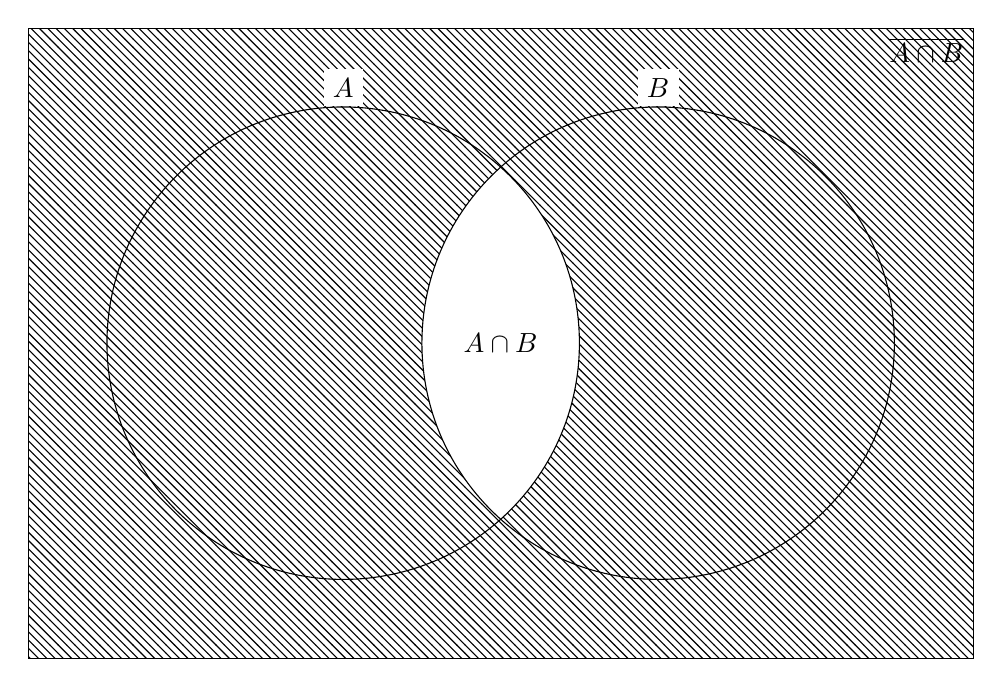
\begin{tikzpicture}
		\def\firstcircle{(-2,0) circle [radius = 3]};
		\def\secondcircle{(2,0) circle [radius = 3]};
		\def\universalrectangle{(-6,-4) rectangle (6,4)};
		
		\begin{scope}
			\fill [pattern = north west lines] \universalrectangle;
			\clip \firstcircle;
			\fill [white] \secondcircle;
		\end{scope}
		
		\begin{scope}
			\draw \firstcircle;
			\draw \secondcircle;
			\draw \universalrectangle;
		\end{scope}
		
		\begin{scope}
			\node [above, fill = white] at (-2,3) {$A$};
			\node [above, fill = white] at (2,3) {$B$};
		\end{scope}
		
		\begin{scope}
			\node at (0,0) {$A \cap B$};
			\node [below left] at (6,4) {$\overline{A \cap B}$};
		\end{scope}
	\end{tikzpicture}
	\caption{$\overline{A \cap B}$}
\end{figure}

\begin{figure}[H]
	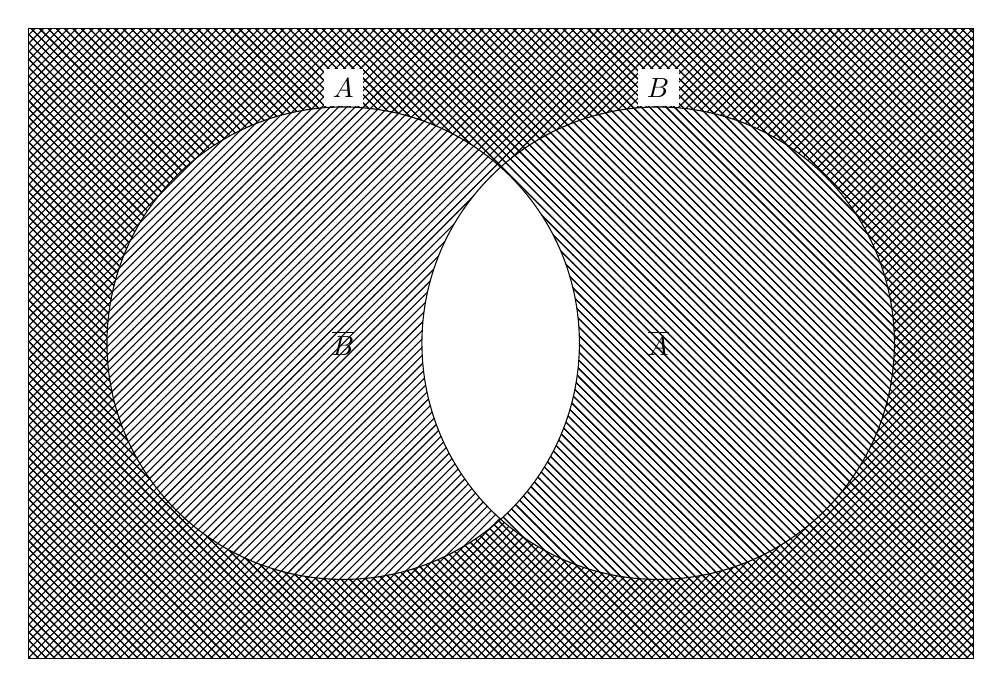
\begin{tikzpicture}
		\def\firstcircle{(-2,0) circle [radius = 3]};
		\def\secondcircle{(2,0) circle [radius = 3]};
		\def\universalrectangle{(-6,-4) rectangle (6,4)};
		
		\begin{scope}
			\fill [pattern = north west lines] \universalrectangle;
			\fill [white] \firstcircle;
		\end{scope}
		
		\begin{scope}
			\clip 
				\universalrectangle
				\firstcircle;
			\fill [pattern = north west lines] \universalrectangle;
		\end{scope}
		
		\begin{scope}
			\clip 
				\universalrectangle
				\secondcircle;
			\fill [pattern = north east lines] \universalrectangle;
		\end{scope}
		
		\begin{scope}
			\draw \firstcircle;
			\draw \secondcircle;
			\draw \universalrectangle;
		\end{scope}
		
		\begin{scope}
			\node [above, fill = white] at (-2,3) {$A$};
			\node [above, fill = white] at (2,3) {$B$};
		\end{scope}
		
		\begin{scope}
			\node at (-2,0) {$\overline{B}$};
			\node at (2,0) {$\overline{A}$};
		\end{scope}
	\end{tikzpicture}
	\caption{$\overline{A} \cup \overline{B}$}
\end{figure}

\strangesection{1.19}{}

\strangesubsection{2}{}

Let
\begin{align*}
	f(x) &= x^2\\
	g(x) &= 2x
\end{align*}
Therefore,
\begin{align*}
	f\left( g(x) \right) &= (2x)^2\\
	&= 4 x^2\\
	g\left( f(x) \right) &= 2 x^2\\
	\therefore f(g(x)) &\neq g(f(x))
\end{align*}
Hence, composition is not commutative.

\strangesection{2.5}{}

\begin{align*}
	| \{ 0,1 \}^k | &= | \{ 0,1 \} \times \{ 0,1 \}^{k - 1}  |\\
	\intertext{For any finite sets $A$, $B$, $| A \times B | = |A| \cdot |B|$. Therefore,}
	| \{ 0,1 \}^k | &= | \{ 0,1 \} | \cdot | \{ 0,1 \}^{k - 1} |\\
	&= | \{ 0,1 \} | \cdot | \{ 0,1 \} | \cdot | \{ 0,1 \}^{k - 2} |\\
	&\quad \vdots\\
	&= \overbrace{| \{ 0,1 \} | \cdot \dots \cdot| \{ 0,1 \}|}^{k \textnormal{ times }}\\
	&= 2^k
\end{align*}

\strangesection{2.6}{}

Let
\begin{align*}
	|A| &= n
\end{align*}
The number of subsets of $A$ is 
\begin{align*}
	&\quad \dbinom{n}{0} + \dbinom{n}{1} + \dots + \dbinom{n}{n - 1} + \dbinom{n}{n}\\
	&= \sum\limits_{r = 0}^{n} \dbinom{n}{r}\\
	&= \sum\limits_{r = 0}^{n} \dbinom{n}{r} 1^r \cdot 1^{n - r}\\
	&= (1 + 1)^n &\textnormal{(by Binomial theorem)}\\
	&= 2^n\\
	&= 2^{|A|}
\end{align*}

\strangesection{2.7}{}

Let
\begin{align*}
	A &= \{a_1, \dots, a_m\}\\
	B &= \{b_1, \dots, b_n\}
\end{align*}
Therefore, $f(a_1)$ can be exactly one out of $b_1, \dots, b_n$. 
Similarly for all $a_2, \dots, a_m$.\\
Therefore, there are $n$ possible combinations for every $a_i \in A$.\\
Therefore, the total number of possible combinations between $A$ and $B$ are $\overbrace{n \cdot \dots \cdot n}^{m \textnormal { times }}$.\\
Therefore,
\begin{align*}
	|F| &= n^m\\
	\therefore |F| &= |B|^{|A|}
\end{align*}
\qed

\end{document}